\documentclass[tikz,border=8pt]{standalone}
\usepackage[T1]{fontenc}
\usepackage{lmodern}
\usepackage{amsmath}
\usepackage{amssymb}
\usetikzlibrary{arrows.meta,positioning,calc,decorations.pathreplacing}
\definecolor{ink}{HTML}{243447}
\definecolor{blue}{HTML}{236A91}
\definecolor{purple}{HTML}{79539B}
\definecolor{teal}{HTML}{247F79}
\definecolor{muted}{HTML}{627080}
% Suggested caption: Hierarchical boundary-token embedding. (A) Each interval
% contributes START and END tokens, irrespective of its duration. (B) Connections
% denote shared hierarchy entries: the state boundary pair shares E_1--E_3,
% while glucose state and trend share E_1. Here t_0 is admission time and t_c
% is the trend start. (C) All four embedding lookups and the Time2Vec vector
% are concatenated and projected into one input vector per boundary token.
% The hierarchy changes representations without adding sequence positions.
\begin{document}
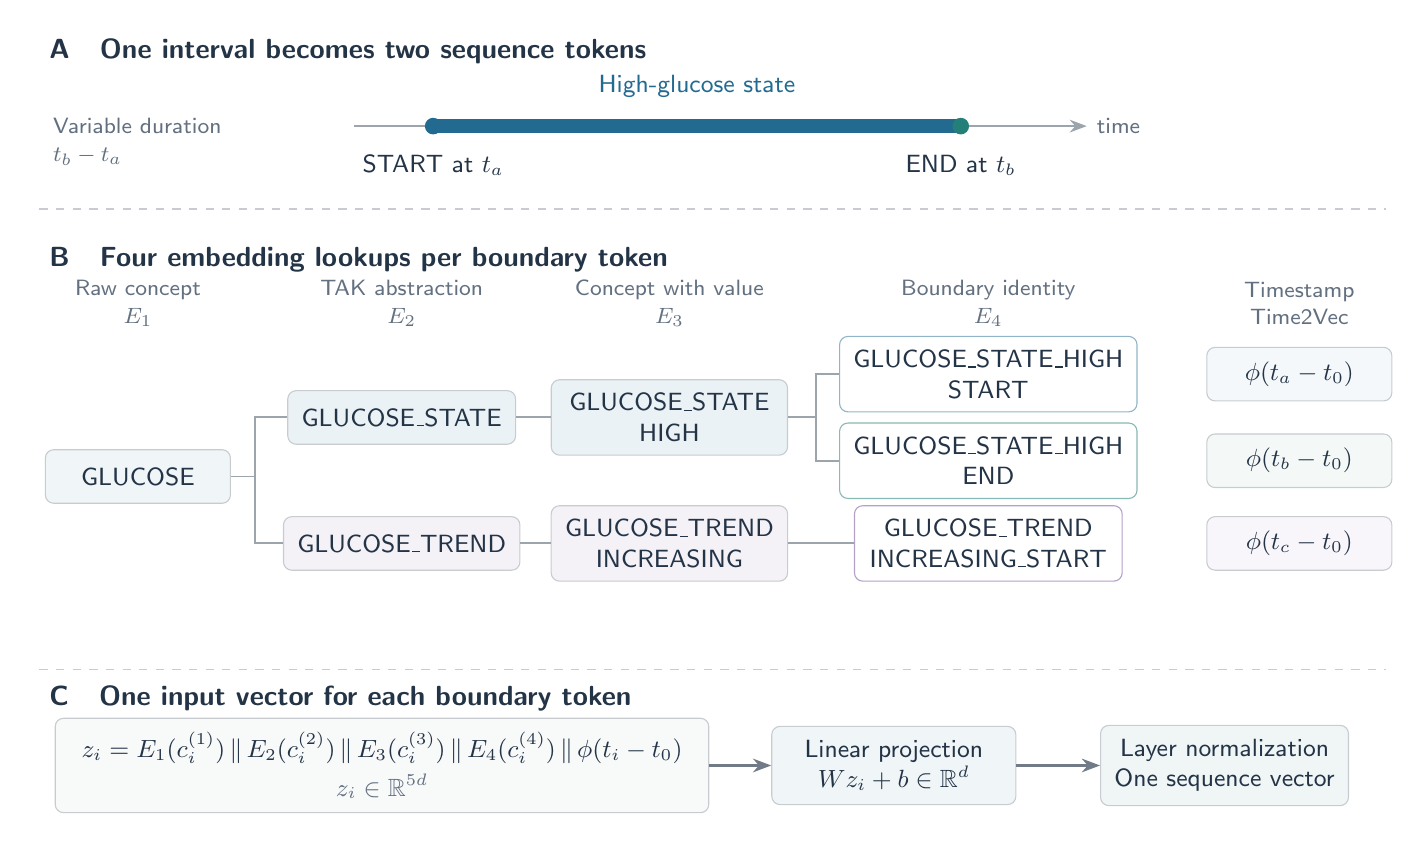
\begin{tikzpicture}[
  x=1cm,y=1cm,font=\sffamily\fontsize{9}{11}\selectfont,
  text=ink,>=Stealth,
  card/.style={draw=ink!25,rounded corners=3pt,fill=white,
    minimum height=0.68cm,align=center,inner sep=5pt},
  link/.style={draw=ink!45,line width=.7pt},
  flow/.style={->,draw=ink!65,line width=.8pt},
  head/.style={font=\sffamily\bfseries\fontsize{10}{12}\selectfont},
  note/.style={text=muted,font=\sffamily\fontsize{8.5}{10}\selectfont,align=center}
]
\path[use as bounding box] (-.15,1.3) rectangle (17.25,-8.8);

% A: the interval contributes boundary tokens, independent of its duration.
\node[head,anchor=west] at (0,1.0) {A\quad One interval becomes two sequence tokens};
\draw[link,->] (4.0,.05) -- (13.3,.05) node[right,note] {time};
\draw[blue,line width=5pt] (5.0,.05) -- (11.7,.05);
\fill[blue] (5.0,.05) circle (3pt);
\fill[teal] (11.7,.05) circle (3pt);
\node[above=7pt,text=blue] at (8.35,.05) {High-glucose state};
\node[below=7pt,align=center] at (5.0,.05) {START at $t_a$};
\node[below=7pt,align=center] at (11.7,.05) {END at $t_b$};
\node[note,anchor=west,align=left] at (.05,-.15) {Variable duration\\$t_b-t_a$};
\draw[draw=ink!25,dashed,line width=.6pt] (0,-1.0) -- (17.1,-1.0);

% B: links indicate common IDs, not a sequence of operations.
\node[head,anchor=west] at (0,-1.65) {B\quad Four embedding lookups per boundary token};
\node[note] at (1.25,-2.2) {Raw concept\\$E_1$};
\node[note] at (4.6,-2.2) {TAK abstraction\\$E_2$};
\node[note] at (8.0,-2.2) {Concept with value\\$E_3$};
\node[note] at (12.05,-2.2) {Boundary identity\\$E_4$};
\node[note] at (16.0,-2.2) {Timestamp\\Time2Vec};

\node[card,fill=blue!7,minimum width=2.35cm] (raw) at (1.25,-4.4) {GLUCOSE};
\node[card,fill=blue!9,minimum width=2.7cm] (state) at (4.6,-3.65) {GLUCOSE\_STATE};
\node[card,fill=purple!8,minimum width=2.7cm] (trend) at (4.6,-5.25) {GLUCOSE\_TREND};
\node[card,fill=blue!9,minimum width=3.0cm] (high) at (8.0,-3.65) {GLUCOSE\_STATE\\HIGH};
\node[card,fill=purple!8,minimum width=3.0cm] (increasing) at (8.0,-5.25) {GLUCOSE\_TREND\\INCREASING};

\node[card,draw=blue!50,minimum width=3.4cm] (ss) at (12.05,-3.1) {GLUCOSE\_STATE\_HIGH\\START};
\node[card,draw=teal!55,minimum width=3.4cm] (se) at (12.05,-4.2) {GLUCOSE\_STATE\_HIGH\\END};
\node[card,draw=purple!55,minimum width=3.4cm] (ts) at (12.05,-5.25) {GLUCOSE\_TREND\\INCREASING\_START};

\draw[link] (raw.east) -- ++(.3,0) |- (state.west);
\draw[link] (raw.east) -- ++(.3,0) |- (trend.west);
\draw[link] (state.east) -- (high.west);
\draw[link] (trend.east) -- (increasing.west);
\draw[link] (high.east) -- ++(.35,0) |- (ss.west);
\draw[link] (high.east) -- ++(.35,0) |- (se.west);
\draw[link] (increasing.east) -- (ts.west);

\node[card,fill=blue!5,minimum width=2.35cm] (timea) at (16.0,-3.1) {$\phi(t_a-t_0)$};
\node[card,fill=teal!5,minimum width=2.35cm] (timeb) at (16.0,-4.2) {$\phi(t_b-t_0)$};
\node[card,fill=purple!5,minimum width=2.35cm] (timec) at (16.0,-5.25) {$\phi(t_c-t_0)$};

\draw[draw=ink!25,dashed,line width=.6pt] (0,-6.85) -- (17.1,-6.85);

% C: five d-dimensional components yield one sequence vector.
\node[head,anchor=west] at (0,-7.22) {C\quad One input vector for each boundary token};
\node[card,fill=ink!3,minimum width=8.3cm] (concat) at (4.35,-8.07)
  {$z_i=E_1(c_i^{(1)})\,\Vert\,E_2(c_i^{(2)})\,\Vert\,E_3(c_i^{(3)})\,\Vert\,E_4(c_i^{(4)})\,\Vert\,\phi(t_i-t_0)$\\[3pt]
  \textcolor{muted}{$z_i\in\mathbb{R}^{5d}$}};
\node[card,fill=blue!7,minimum width=3.1cm] (project) at (10.85,-8.07)
  {Linear projection\\$Wz_i+b\in\mathbb{R}^{d}$};
\node[card,fill=teal!7,minimum width=3.0cm] (output) at (15.05,-8.07)
  {Layer normalization\\One sequence vector};
\draw[flow] (concat.east) -- (project.west);
\draw[flow] (project.east) -- (output.west);
\end{tikzpicture}
\end{document}
